\documentclass[10pt]{beamer}
\usetheme[
%%% option passed to the outer theme
%    progressstyle=fixedCircCnt,   % fixedCircCnt, movingCircCnt (moving is deault)
  ]{Feather}
  
% If you want to change the colors of the various elements in the theme, edit and uncomment the following lines

% Change the bar colors:
%\setbeamercolor{Feather}{fg=red!20,bg=red}

% Change the color of the structural elements:
%\setbeamercolor{structure}{fg=red}

% Change the frame title text color:
%\setbeamercolor{frametitle}{fg=blue}

% Change the normal text color background:
%\setbeamercolor{normal text}{fg=black,bg=gray!10}

\usefonttheme[onlymath]{serif}

%-------------------------------------------------------
% INCLUDE PACKAGES
%-------------------------------------------------------

\usepackage[utf8]{inputenc}
\usepackage[english]{babel}
\usepackage[T1]{fontenc}
\usepackage{helvet}
\usepackage{mathtools}
\usepackage{amsmath,amssymb}
\usepackage{smartdiagram}

%\usepackage{animate}
\usepackage{graphicx}

\usepackage{multimedia}

\usepackage{animate}

\usepackage{mathtools}
\graphicspath{ {images/}, {gif/} }

\usepackage[most]{tcolorbox}
\usepackage[absolute,overlay]{textpos}

%\usepackage{media9}
\usepackage{tikz}
%-------------------------------------------------------
% DEFFINING AND REDEFINING COMMANDS
%-------------------------------------------------------

% colored hyperlinks
\newcommand{\chref}[2]{
  \href{#1}{{\usebeamercolor[bg]{Feather}#2}}
}

%-------------------------------------------------------
% INFORMATION IN THE TITLE PAGE
%-------------------------------------------------------

\title[Driven Wheelchair Project] % [] is optional - is placed on the bottom of the sidebar on every slide
{ % is placed on the title page
      \textbf{EMG - Driven Wheelchair Project}
}


\author[Erivelton Gualter]
{      Erivelton Gualter dos Santos \\
      {\ttfamily erivelton.gualter@gmail.com}
}

\subtitle[https://eriveltongualter.github.io/]{}

\institute[]
{
      FEI University\\
      São Bernardo do Campo, São Paulo - Brazil\\
  
  %there must be an empty line above this line - otherwise some unwanted space is added between the university and the country (I do not know why;( )
}

\date{\today}

%-------------------------------------------------------
% THE BODY OF THE PRESENTATION
%-------------------------------------------------------

\begin{document}

%-------------------------------------------------------
% THE TITLEPAGE
%-------------------------------------------------------

{\1% % this is the name of the PDF file for the background
\begin{frame}[plain,noframenumbering] % the plain option removes the header from the title page, noframenumbering removes the numbering of this frame only
  \titlepage % call the title page information from above
\end{frame}}


\begin{frame}{Content}{}
\tableofcontents
\end{frame}

%-------------------------------------------------------
\section{Introduction}
%-------------------------------------------------------
\subsection{Overview Projects}
\begin{frame}{Introduction}{Overview Projects}
\begin{itemize}[<+->]
	\item B.S. Automation and Control Engineer at FEI University.
	%\item<2-> Tutoring experience in: Physics I and Differential and Integral Calculus II.
	\item Undergraduate Researcher at Robotic and Artificial Intelligence Laboratory.	
	\begin{figure}
		\includegraphics[width=0.6\linewidth]{robo.jpg}	
	\end{figure}
\end{itemize}
\end{frame}
%-------------------------------------------------------
\begin{frame}{Introduction}{Overview Projects}
	\begin{figure}
	\centering
	\includegraphics[width=1\linewidth]{game.png}
	\end{figure}
\end{frame}
%-------------------------------------------------------
\begin{frame}{Introduction}{Overview Projects}
\begin{itemize}
	\item Machining and fabrication experience. 
	\begin{figure}
	\centering
	\animategraphics[loop,autoplay,height=6cm]{1}{mec-}{1}{16}		
	\end{figure}
\end{itemize}
\end{frame}
%-------------------------------------------------------
\begin{frame}{Introduction}{Overview Projects}
\begin{columns}
\column{0.5\textwidth}
\begin{minipage}[c][0.3\textheight][c]{\linewidth}
\begin{itemize}
	\item Path Planner Algorithms: Dijkstra, A* Grid and Probabilistic Roadmap (PRM).
\end{itemize}
\end{minipage}
\begin{minipage}[c][0.4\textheight][c]{\linewidth}
  \centering
  \animategraphics[loop,autoplay,height=4.3cm]{90}{sixlink-}{0}{122}	
\end{minipage}
\column{0.5\textwidth}
\begin{minipage}[c][0.4\textheight][c]{\linewidth}
	\centering
  \animategraphics[loop,autoplay,height=3.8cm]{45}{DijkstraGrid-}{0}{78}	
\end{minipage}
\begin{minipage}[c][0.4\textheight][c]{\linewidth}
  \centering
  \animategraphics[loop,autoplay,height=3.8cm]{45}{AStarGrid-}{0}{19}	
\end{minipage}
\end{columns}
\end{frame}


%-------------------------------------------------------
\subsection{Assistive Technology Research Center}
%-------------------------------------------------------
\begin{frame}{Introduction}{Assistive Technology Research Center}
%-------------------------------------------------------
\begin{itemize}
	\item The group is formed by different departments, such as the Mechanical, Electrical and Computer Science department. 
	\item Also, has collaborations with biomedical departments from Federal University of ABC:
	\begin{figure}
		\includegraphics[width=0.6\linewidth]{BMClab.png}
	\end{figure}
	\item Create National Assistive Tecnology aimed the power-assisted wheelchair. 
\end{itemize}
\end{frame}

\begin{frame}{Assistive Technology Research Center}{NTA “Núcleo de Tecnologia Assistiva”}
%-------------------------------------------------------
\begin{figure}
\centering
\includegraphics[width=0.8\linewidth]{propulsion.jpg}
\caption{Biomechanics and Motor Control Laboratory}
\end{figure}
\end{frame}

%-------------------------------------------------------
\subsection{Motivation}
\begin{frame}{Motivation}{Numbers}
\begin{itemize}
	\item 45.6 million people have some kind of disability.
	\item 14 million Brazilians have some kind of motor deficiency.
	\item 5 million are wheelchair users.
	\item 1 to 2\% of the planet's population depends on a wheelchair.
\end{itemize}
\end{frame}


%-------------------------------------------------------
\subsection{Wheelchair}
\begin{frame}{Wheelchair}{Classification}
%-------------------------------------------------------
\begin{columns}
\column{0.33\textwidth}
\begin{minipage}[c][0.5\textheight][c]{\linewidth}
  \centering
  \includegraphics<1->[width=0.9\linewidth]{wc-manual.jpg}
  \begin{itemize}
  \item<1-> Mechanically simpler and lighter;
  \item<1-> Allow Physical activity;
  \item<1-> Low Cost.
  \end{itemize}
\end{minipage}

\column{0.33\textwidth}
\begin{minipage}[c][0.4\textheight][c]{\linewidth}
  \centering
  \includegraphics<2->[width=0.9\linewidth]{wc-motorized.jpg}
  \begin{itemize}
  \item<2-> Heavy structure;
  \item<2-> Hard to carry;
  \item<2-> Users are those who suffered high injury in the spinal cord.
  \end{itemize}
\end{minipage}

\column{0.33\textwidth}
\begin{minipage}[c][0.4\textheight][c]{\linewidth}
	\centering
  \includegraphics<3->[width=0.9\linewidth]{wc-hybrid.jpg}
  \begin{itemize}
  \item<3-> Operates like a M.W.;
  \item<3-> User accomplish more with less effort;
  \item<3-> Navigate uneven surfaces.
  \end{itemize}
\end{minipage}

\end{columns}
\end{frame}


%-------------------------------------------------------
\section{Modeling Driven Wheelchair}
\begin{frame}{Modeling Driven Wheelchair}{Design Workflow}
%-------------------------------------------------------
\begin{enumerate}
	\item<1-> Brainstorm: Set the features of the wheelchair
	\begin{itemize}
		\item<1-> Compensate the force of gravity on a hill;
		\item<1-> Propose new control techniques;
		\item<1-> Wheelchair wheelie to overcome obstacle.
	\end{itemize}
	\item<2-> Experiments: Estimate parameters of a manual wheelchair to estimate the motor characteristic.
	\begin{itemize}[<+->]
		\item<2-> Center of Mass;
		\item<2-> Moment of Inertia;
		\item<2-> Minimum Torque to lift-off the wheelchair.
	\end{itemize}
	\item<3-> Modeling: CAD Wheelchair Drawing
	\item<4-> Build: Manufacture the prototype
	\item<5-> Electronic: Manufacture Electronic Boards
	\item<6-> Control: Control device.
\end{enumerate}

\end{frame}

\subsection{Overview Wheelie}
%-------------------------------------------------------
\begin{frame}{Project}{Overview Wheelie}
%-------------------------------------------------------
\centering
\includegraphics[width=0.6\linewidth]{wheelie2.png} \\
\includegraphics[width=0.6\linewidth]{wheelie1.png} \\ 
\begin{figure}
\includegraphics[width=0.6\linewidth]{wheelie3.png}
\caption{Wheelie manuever. (Denison, 2013)}
\end{figure}
\end{frame}
%-------------------------------------------------------
\begin{frame}{Introduction}{Wheelchair wheelie}
%-------------------------------------------------------
\begin{figure}
\centering
\includegraphics[width=0.7\linewidth]{stairs.png}
\caption{Wheelie in stairs.}
\end{figure}
\end{frame}
%-------------------------------------------------------
\begin{frame}{Introduction}{Wheelchair wheelie}
%-------------------------------------------------------
\begin{figure}
\centering
\includegraphics[width=0.7\linewidth]{descend.png}
\caption{Wheelie in descend terrains.}
\end{figure}
\end{frame}

\subsection{Modeling Driven Wheelchair}
\begin{frame}{Driven Wheelchair Design}{Model of Phase 1}
%-------------------------------------------------------
\begin{columns}
\column{0.3\textwidth}
\begin{minipage}[c][0.4\textheight][c]{\linewidth}
  \centering
  \includegraphics[width=0.7\linewidth]{phase1.png}
\end{minipage}
\begin{minipage}[c][0.4\textheight][c]{\linewidth}
  \centering
  \includegraphics[width=1.1\linewidth]{phase1.JPG}
\end{minipage}
\column{0.5\textwidth}
\begin{minipage}[c][0.4\textheight][c]{\linewidth}
  \begin{itemize}
  \item Sagittal Plane (2D);
  \item 2 rigid bodies;
  \item Front wheels on the ground \textcolor{red}{(stable)};
  \item 1 DoF; 
  \item Control: wheel torque;
  \item Equation of Motion:
 	\begin{eqnarray*}
 		\frac{\tau}{R} = \left( M + \frac{J_R}{R^2} \right)\ddot{x} + F_R
 	\end{eqnarray*}   
  \item Transition Acceleration:
 	\begin{eqnarray*}
 		\ddot{x_{nf}} = \frac{d_{xcg}}{h_{cg}}g
 	\end{eqnarray*}   
  \end{itemize}
\end{minipage}
\end{columns}
\end{frame}
%-------------------------------------------------------
\begin{frame}{Driven Wheelchair Design}{Model of Phase 2}
%-------------------------------------------------------
\begin{columns}
\column{0.3\textwidth}
\begin{minipage}[c][0.4\textheight][c]{\linewidth}
  \centering
  \includegraphics[width=0.7\linewidth]{phase2.png}
\end{minipage}
\begin{minipage}[c][0.4\textheight][c]{\linewidth}
  \centering
  \includegraphics[width=0.9\linewidth]{phase2.jpg}
\end{minipage}
\column{0.7\textwidth}
\begin{minipage}[c][0.4\textheight][c]{\linewidth}
  \begin{itemize}
  \item Sagittal Plane (2D);
  \item 2 rigid bodies;
  \item Front wheels off the ground \textcolor{red}{(unstable)};
  \item 2 DoF's; 
  \item Control: wheel torque;
  \item Equations of Motion:

\begin{eqnarray*}
  \begin{matrix}
  \resizebox{1\textwidth}{!} 
{
    $ \tau - F_rR = \left[J_R + \left(M_r + M_c \right)R^2 \right]\ddot{\theta} + \left(M_cRlcos(\phi) \right)\ddot{\phi} - \left(M_cRl\dot{\phi}^2sin(\phi) \right) $
} 
\\
  \resizebox{.8 \textwidth}{!}%
{
    $ -\tau = \left( M_c Rl cos(\phi)\right)\ddot{\theta} + \left(J_c+M_cl^2 \right)\ddot{\phi} -M_cglsin(\phi) $
}   
  \end{matrix}
  \end{eqnarray*}
  
  \end{itemize}
\end{minipage}
\end{columns}
\end{frame}


%-------------------------------------------------------
\begin{frame}{Driven Wheelchair Design}{Lift-Off Torque}
%-------------------------------------------------------
\begin{eqnarray*}
\begin{matrix}
	\frac{\tau}{R} = \left( M + \frac{J_R}{R^2} \right)\ddot{x} + F_R \\
	\\
	\ddot{x_{nf}} = \frac{d_{xcg}}{h_{cg}}g
\end{matrix} \Bigg\}
	\tau_{nf} = \left[ \left( M + \frac{J_R}{R^2} \right)\frac{d_{xcg}}{h_{cg}}g + F_R \right]R \\
\end{eqnarray*}   

\begin{columns}[T] % align columns
\begin{column}{.4\textwidth}
%\color{red}\rule{\linewidth}{4pt}
  \centering
  \includegraphics[width=1.0\linewidth]{phase1.JPG}
\end{column}%
\hfill%
\begin{column}{.70\textwidth}
%\color{blue}\rule{\linewidth}{4pt}
  \centering
  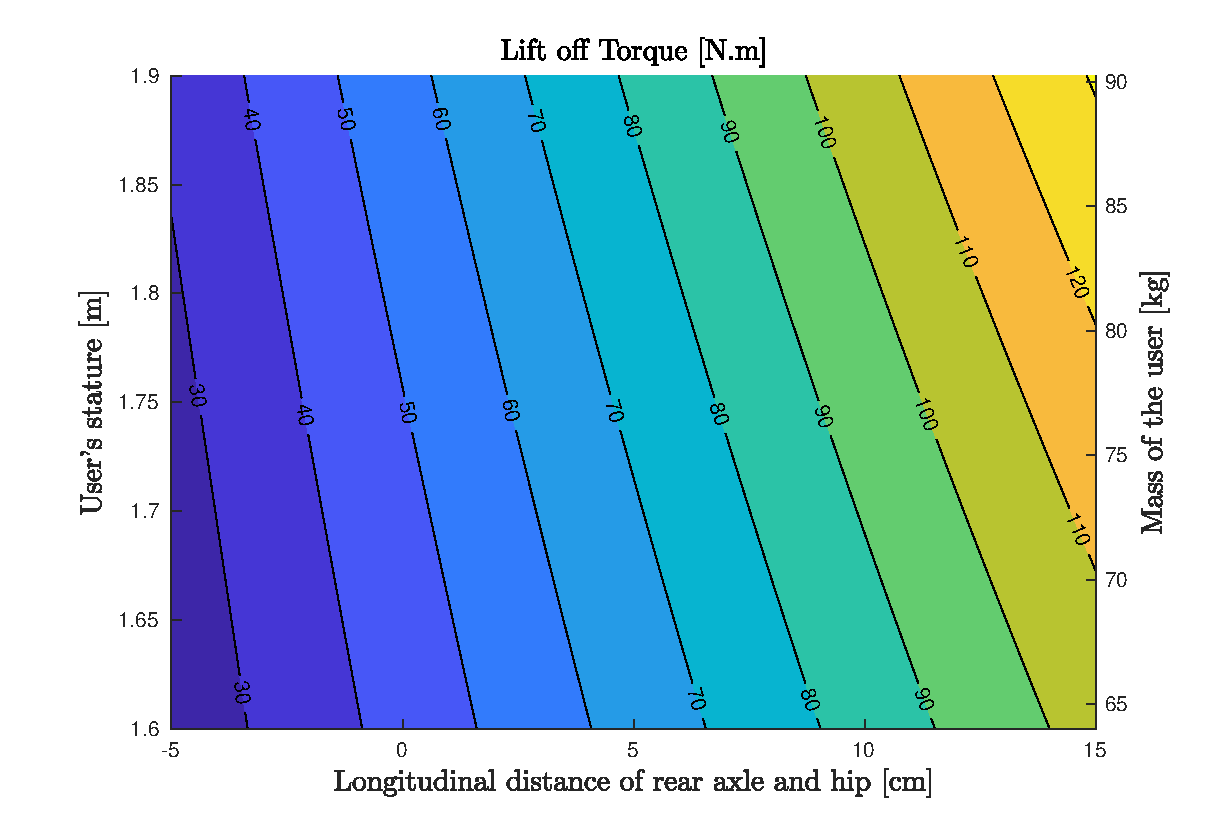
\includegraphics[width=0.9\linewidth]{torque}
\end{column}%
\end{columns}
\end{frame}

%-------------------------------------------------------
\begin{frame}{Driven Wheelchair Design}{Estimation of Parameters}
%-------------------------------------------------------
\begin{columns}
\column{0.6\textwidth}
\begin{minipage}[c][0.4\textheight][c]{\linewidth}
  \begin{figure}
  \includegraphics[width=1\linewidth]{CG_wheel.png}
  \caption{Suspended Experiment}
  \end{figure}
\end{minipage}
\begin{minipage}[c][0.4\textheight][c]{\linewidth}
  \centering
  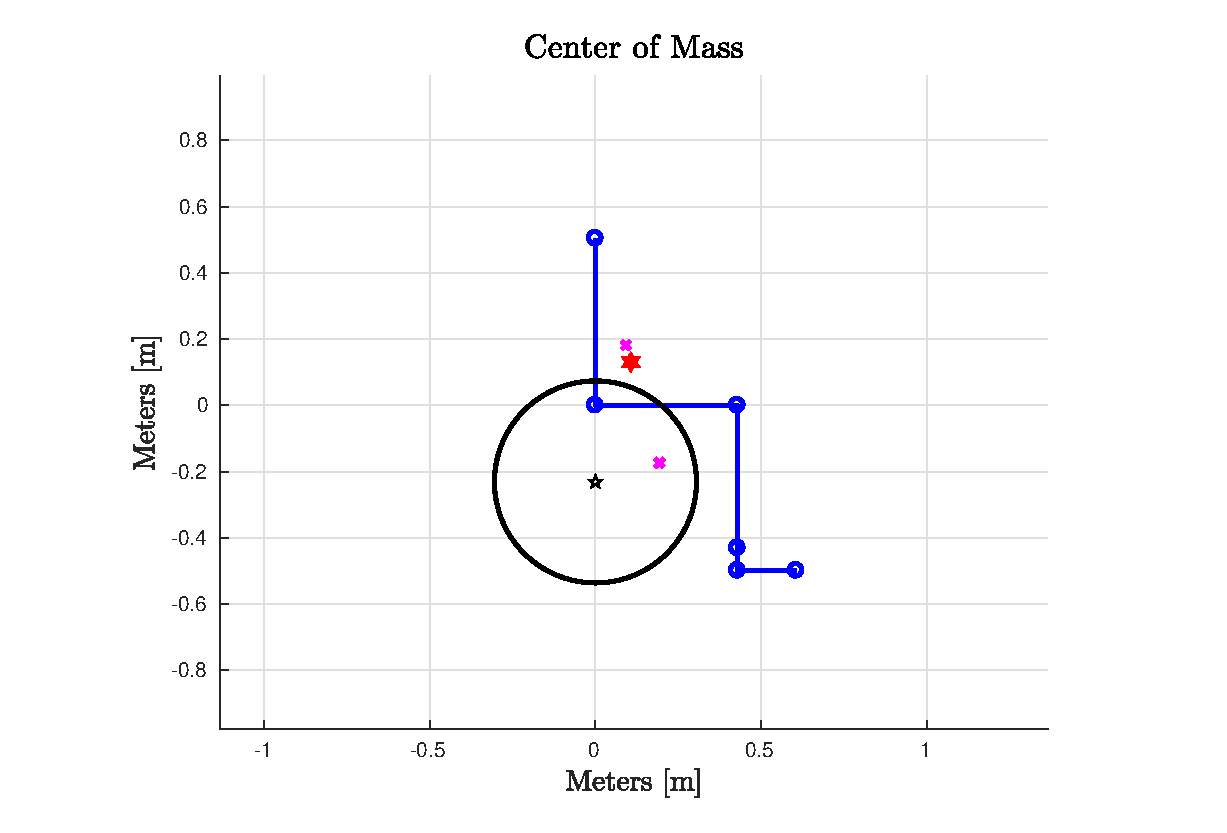
\includegraphics[width=0.9\linewidth]{CG}
\end{minipage}
\column{0.4\textwidth}
\begin{minipage}[c][0.1\textheight][c]{\linewidth}
	\centering
		Center of Mass
\end{minipage}
\begin{minipage}[c][0.6\textheight][c]{\linewidth}
  \centering
  \begin{figure}
  \includegraphics[width=0.9\linewidth]{winter.png}
  \caption{(Winter, 2009)}
  \end{figure}
\end{minipage}
\end{columns}
\end{frame}

\section{Estimation of Parameters} 
%-------------------------------------------------------
\begin{frame}{Driven Wheelchair Design}{Estimation of Parameters}
%-------------------------------------------------------
\begin{columns}
\column{0.5\textwidth}
\begin{minipage}[c][0.3\textheight][c]{\linewidth}
  \centering
	Moment of Inertia
  \end{minipage}
\begin{minipage}[c][0.4\textheight][c]{\linewidth}
  \begin{figure}
  \includegraphics[width=0.9\linewidth]{winter.png}
  \end{figure}
\end{minipage}
\column{0.5\textwidth}
\begin{minipage}[c][0.45\textheight][c]{\linewidth}
  \begin{figure}
  \centering
  \includegraphics[width=0.8\linewidth]{momentwc1.jpg}
  \caption{Oscillation Experiment}
  \end{figure}
\end{minipage}
\begin{minipage}[c][0.4\textheight][c]{\linewidth}
  \centering
  \includegraphics[width=1\linewidth]{pendulumwheel.png}
\end{minipage}
\end{columns}
\end{frame}


%-------------------------------------------------------
\begin{frame}{Driven Wheelchair Design}{Project Drawing}
%-------------------------------------------------------
\begin{columns}[T] % align columns
\begin{column}{.4\textwidth}
\color{red}\rule{\linewidth}{3pt}
  \begin{itemize}
  \item BLDC Motors 36V;
  \item SBL1360 60V 1x20A Brushless DC Motor Controller;
  \item Arduino Mega 2560 Microcontroller Rev3;
  \item MPU6050 3 Axis Accelerometer Gyroscope.
  \end{itemize}
\color{red}\rule{\linewidth}{3pt}
\end{column}%
\hfill%
\begin{column}{.58\textwidth}
%\color{blue}\rule{\linewidth}{4pt}
  \animategraphics[loop,autoplay,width=8cm]{5}{animate_}{0}{40}
  \end{column}%
\end{columns}
\end{frame}
%-------------------------------------------------------
\begin{frame}{Driven Wheelchair Design}{Project Drawing}
%-------------------------------------------------------
\begin{columns}[T] % align columns
\begin{column}{.3\textwidth}
  \centering
  \includegraphics<1->[width=1\linewidth]{wheelchair_final.jpg}
\end{column}%
\begin{column}{.3\textwidth}
  \centering
  \includegraphics<1->[width=1\linewidth]{fork2.png}
\end{column}%
\begin{column}{.3\textwidth}
	\begin{itemize}
	  \item BDLC Motors 36V;
	  \item Arduino Mega 2560;
	  \item Lithium Battery 10Ah;
	  \item Fork structure.
	\end{itemize}
\end{column}%
\end{columns}
\end{frame}

\section{Controller}
\subsection{Tips of Biomedical sensors}
%-------------------------------------------------------
\begin{frame}{Controller}{HMI}
%-------------------------------------------------------
\begin{columns}
\column{0.5\textwidth}
\begin{minipage}[c][0.2\textheight][c]{\linewidth}
  \begin{itemize}
  \item There are several approaches of Human-Machine Interfaces to control a wheelchair using electro-
biological signals.
  \end{itemize}
  \end{minipage}
\begin{minipage}[c][0.4\textheight][c]{\linewidth}
  \centering
  \includegraphics<1->[width=0.8\linewidth]{wc_emg.jpg}
\end{minipage}
\column{0.5\textwidth}
\begin{minipage}[c][0.4\textheight][c]{\linewidth}
	\centering
  \includegraphics<2->[width=0.4\textheight]{wc_eoc.jpg}
\end{minipage}
\begin{minipage}[c][0.4\textheight][c]{\linewidth}
  \centering
  \includegraphics<3->[width=1\linewidth]{wc_eec.jpg}
\end{minipage}
\end{columns}
\end{frame}

\subsection{EMG sensor}
%-------------------------------------------------------
\begin{frame}{Controller}{EMG Board}
%-------------------------------------------------------
  \begin{itemize}
  	\item The myoletric signal originates in the region of the brain and is transmitted through the central and peripheral nervous system to the muscle.
\begin{figure}
\centering
\includegraphics[width=0.8\linewidth]{illustrationwc.png}
\end{figure}
  \end{itemize}  
\end{frame}
%-------------------------------------------------------
\begin{frame}{Controller}{EMG Board}
%-------------------------------------------------------
	\begin{figure}
	\centering
	\includegraphics[width=0.8\linewidth]{board1.png}
	\caption{Electronic board for the EMG acquisition.}
	\end{figure}
	
	\begin{itemize}
		\item INA121 - Amplifier capable of high gains;
		\item UFA42 - High pass filter (20Hz);
		\item Low pass filter (500Hz);
		\item Notch filter 60Hz.
	\end{itemize}
\end{frame}
%-------------------------------------------------------
\begin{frame}{Controller}{MyoWare Muscle Sensor}
%-------------------------------------------------------
\begin{itemize}
	\item Single-supply voltage of +3.1V to +5V;
	\item Indicador LEDs;
	\item Two Output modes: EMG Envelope and Raw EMG;
	\item Adjustable Gain;
	\item Electrodes snap directly to MyoWare.
\end{itemize}
\animategraphics[loop,autoplay,height=3cm]{5}{board_setup-}{0}{75}
\animategraphics[loop,autoplay,height=3cm]{5}{boardmyo-}{0}{26}
\end{frame}
%-------------------------------------------------------
\begin{frame}{Controller}{MyoWare Muscle Sensor}
%-------------------------------------------------------
	\begin{figure}
	\centering
	\includegraphics[width=0.5\linewidth]{biceps.png}
	\caption{Setup EMG sensors}
	\end{figure}
\end{frame}
%-------------------------------------------------------
\begin{frame}{Controller}{Main View}
%-------------------------------------------------------
	\begin{figure}
	\centering
	\includegraphics[width=1\linewidth]{new_circuit.png}
	\caption{Power and Control Circuit}
	\end{figure}
\end{frame}

\section{Conclusion}
\subsection{Video}
%-------------------------------------------------------
\begin{frame}{Driven Wheelchair}{Video}
%-------------------------------------------------------
\centering
\includegraphics[width=1\linewidth]{promo.png}
\end{frame}

\subsection{Repository and informations}
\begin{frame}{Repository and Informations}{https://eriveltongualter.github.io/}
\vspace*{0.2cm}
\hspace*{-0.5cm}\includegraphics[width=1.1\textwidth,natwidth=100,natheight=87]{webpage.png}
\end{frame}

{\1
\begin{frame}[plain,noframenumbering]
	\finalpage{Thank you}   
\end{frame}}

\end{document}
